\documentclass[11pt]{article}
\usepackage[margin=1in]{geometry}
\usepackage{microtype}
\usepackage{amsmath,amssymb}
\usepackage{booktabs}
\usepackage{array}
\usepackage{graphicx}
\usepackage{enumitem}
\usepackage{xcolor}
\usepackage{hyperref}
\usepackage{natbib}
\usepackage{tikz}
\usetikzlibrary{arrows.meta,positioning,shapes.geometric}
\setlist[itemize]{label=$\bullet$}
\hypersetup{
  colorlinks=true,
  linkcolor=blue!55!black,
  citecolor=blue!55!black,
  urlcolor=blue!55!black,
  pdftitle={Engineering Collective Forecasting: Turning Distributed Engineering Knowledge into Auditable Probabilistic Evidence},
  pdfauthor={Guillaume Harbonnier}
}
\title{Engineering Collective Forecasting:\\Turning Distributed Engineering Knowledge into Auditable Probabilistic Evidence}
\author{Guillaume Harbonnier\\\textit{Independent Researcher}\\\url{https://github.com/gharbonnier78}}
\date{Protocol preprint -- 27 September 2026}

\newcommand{\BS}{\mathrm{BS}}
\newcommand{\logitop}{\operatorname{logit}}
\newcommand{\sigmoid}{\operatorname{logistic}}

\begin{document}
\maketitle
\begin{abstract}
Engineering decisions often depend on information distributed across technical and operational actors and only partly represented in structured project data. This protocol asks whether that distributed knowledge can become auditable probabilistic evidence \emph{beyond what the organization already knows}, without perturbing the engineering process being observed. Study~0 applies a minimum-sufficient-mechanism principle. Study~0A is a dry funnel that tests whether real engineering events can be prospectively converted into important, uncertain, objectively resolvable and confidentiality-safe Forecast Contracts. Study~0B, only if warranted, uses private probability elicitation: the accountable owner's private probability and official status, independent participant forecasts plus meta-predictions, and---where a defensible historical reference class exists---a base-rate forecast are frozen at the same information time. No collective aggregate is exposed before resolution. The primary comparison is the paired Brier-loss difference between a prospectively fixed private collective aggregator and the owner's forecast; base-rate skill is a required secondary reference only for contracts with a defensible historical reference class, and dependence is handled at the operational-cluster level. Prediction markets are deferred to a later intervention-aware study. Design simulations characterize the continuation rule as a screening/non-inferiority gate rather than a superiority test. No empirical forecasting-benefit or operational-value claim is made at protocol stage.
\end{abstract}

\section{Motivation}
Complex engineering programs rarely possess a single complete view of readiness. Integration, test, environment, product and operational actors can hold different pieces of information, some documented and some local or recent. The first scientific question is therefore not which sophisticated mechanism should aggregate that information, but whether a prospectively measurable distributed signal exists at all.

The bounded research question is:

\begin{quote}
Can distributed engineering knowledge be transformed into calibrated, auditable and incrementally useful probabilistic evidence beyond institutional knowledge, without materially interfering with the engineering process being observed?
\end{quote}

Incremental usefulness requires an explicit comparator. Study~0 therefore records, at the same freeze time, an accountable owner's private probability, the existing official status and the private collective forecasts, plus a historical reference-class probability wherever one can be defined prospectively without outcome-driven selection.

\section{Protocol contributions}
This work contributes a prospective protocol rather than an empirical performance result. Its main methodological contributions are:

\begin{itemize}
  \item a project-local \emph{Forecast Contract} that freezes the forecasted event, timing, resolution rule, authoritative evidence, institutional references and safeguards before the outcome is known;
  \item a minimum-sufficient two-stage design in which Study~0A first qualifies whether usable engineering forecast contracts exist, before Study~0B introduces any participant forecasting;
  \item a same-time comparison of a private collective signal with an accountable owner's private forecast, while preventing pre-resolution aggregate exposure and preserving actor/observer and data-custody boundaries;
  \item a reproducible probabilistic evaluation plan using a fixed aggregation rule, normalized binary Brier loss, cluster-aware uncertainty and an explicitly bounded continuation rule.
\end{itemize}

These contributions define an auditable way to test the existence and incremental value of distributed engineering forecasts. They do not establish that collective forecasting is superior to institutional judgment, that the chosen aggregator is optimal, or that exposing forecasts would improve engineering decisions.

\section{The Forecast Contract}
A prediction is auditable only if its meaning and resolution are fixed before the answer is known. Howard's clarity-test tradition motivates the general requirement that an uncertain event be stated so that later observation can settle it without semantic renegotiation \citep{howard1988}. We introduce the project-local object
\[
\mathcal F_j=(Q_j,\Omega_j,T_j,R_j,E_j,A_j,B_j,C_j,X_j,S_j),
\]
where $Q_j$ is the question, $\Omega_j$ the outcome space, $T_j$ the timing contract, $R_j$ the resolution rule, $E_j$ the authoritative evidence, $A_j$ the resolver role, $B_j$ the institutional-reference definition, $C_j$ shared context, $X_j$ exclusions and $S_j$ safeguards.

\textbf{Forecast Contract} is local project terminology, not an external standard.

A good candidate must be important, uncertain at the intended freeze time, objectively resolvable, compatible with an authoritative evidence source, confidentiality-safe and suitable for non-interfering observation.

\section{Related work}

\subsection{Prediction markets and direct probability elicitation}
Prediction markets provide one mechanism for aggregating distributed beliefs, with early organizational applications including sales forecasting and internal corporate markets \citep{chenplott2002,cowgill2009,cowgill2015}. Field evidence also documents departures from an idealized independent-information market, including optimism and correlated trading within organizational and social structures \citep{cowgill2009}. Direct probability elicitation is therefore a substantive comparator rather than a procedural placeholder: prediction polls can retain considerable information and in some settings compete closely with market forecasts \citep{atanasov2017,dana2019}. Study~0 starts with private elicitation because its first question concerns the existence of a distributed engineering signal, not the residual value of a market mechanism.

\subsection{Shared information, meta-predictions and aggregation}
Collective forecasts can be distorted by shared information and correlated errors. A simple probability average is transparent but can be conservative when individual forecasters each condition on only part of the available evidence \citep{baron2014,satopaa2014}. Meta-belief approaches ask respondents not only for their own judgment but also for a prediction of others' judgments. Bayesian Truth Serum introduced second-order population predictions as part of an incentive-compatible elicitation mechanism for subjective data \citep{prelec2004}. The Surprisingly Popular principle later used predicted population responses to recover minority knowledge in single-question crowd-wisdom problems \citep{prelec2017}. Related work uses meta-predictions to adjust for shared information or identify latent expertise without a long individual performance history \citep{palley2019,martinie2020,wilkening2022,peker2025}.

These methods differ in assumptions, targets and algorithms. The fixed logit recalibration in Study~0 is therefore treated as a project-specific, prospectively frozen aggregator inspired by this literature, not as an implementation of Bayesian Truth Serum, Surprisingly Popular, or any cited meta-belief algorithm.

\subsection{Expert judgment in software engineering}
Expert judgment is also an established object of empirical software-engineering research. J{\o}rgensen's review documents extensive use and study of expert estimation for software development effort \citep{jorgensen2004}. That literature motivates taking the accountable engineering owner's judgment seriously as an institutional comparator rather than benchmarking a crowd only against an empty or purely statistical baseline. The target here is different---short-horizon engineering qualification outcomes rather than development effort---so no performance result is transferred from effort-estimation studies.

\subsection{Measurement reactivity and the interference problem}
Elicitation itself need not be behaviorally inert. A meta-analysis of intention and self-prediction questions reports a small average question--behavior effect across behavioral studies \citep{wood2016}. The domains and interventions differ materially from engineering work, so the reported effect size is not imported into this protocol. Instead, the literature supplies a general validity warning: asking an actor to predict an outcome may change attention or behavior. This motivates private elicitation, pre-resolution aggregate suppression, explicit actor/observer metadata and a separate detected-interference sensitivity analysis.

\subsection{Position of the present protocol}
The protocol combines these strands around a narrower engineering question: whether private distributed forecasts add probabilistic information beyond a same-time accountable-owner signal under prospectively resolvable evidence contracts. It does not treat prediction markets, meta-predictions or expert judgment as inherently superior. Its distinguishing object is the coupling of forecast semantics, institutional comparators, authoritative outcome evidence and non-interference safeguards in a single prospective engineering protocol.

\section{Study 0 design}

\subsection{Study 0A: dry contract funnel}
Study~0A runs before participant forecasting. During a frozen 4--6 week intake window, candidate events from predeclared engineering families are logged prospectively. No market and no forecast participants are used. Each candidate is evaluated for importance, uncertainty, resolvability, authoritative evidence, confidentiality safety and non-interference suitability. Base-rate availability is recorded but is not itself an admission criterion.

Passing candidates are frozen as Forecast Contracts and later resolved using their declared evidence. Study~0A estimates the candidate-to-admissible and admissible-to-clean-resolution fractions. Before intake, the protocol freezes a minimum admissible yield, a minimum clean-resolution rate and a maximum projected time to reach the Study~0B structural targets. The default protocol values are 0.30, 0.80 and 26 weeks respectively, with $J_{min}=30$ contracts and $K_{min}=8$ independent clusters. Candidate actor/observer pool counts and drafting effort are collected without participant forecasting. This is the primary feasibility test.

\subsection{Study 0B: private forecasting}
Study~0B starts only if Study~0A and governance gates justify continuation. At a common freeze time $T_f$, the study captures:
\[
p_j^{\mathrm{base}},\qquad
p_j^{\mathrm{owner}},\qquad
s_j^{\mathrm{official}},\qquad
\{p_{ij},m_{ij}\}_{i=1}^{n_j}.
\]
The first term is present when a defensible historical base rate exists, the second is the accountable owner's private probability, the third is the existing official status, and the final pair contains each participant's own probability and expected peer-average probability. Absence of a defensible base rate does not remove an otherwise-admissible contract from the primary crowd-versus-owner comparison.

No participant sees another forecast, the base rate, owner forecast or any aggregate before resolution. The data custodian also hides aggregates from any study-team member with decision authority over the contract. Eligible forecasters must have role-relevant knowledge of the event, its generating process or its evidence path; uninformed observers cannot be recruited merely to satisfy a quota. The accountable owner may also forecast only if independently eligible, but the primary crowd aggregate excludes that owner and an including-owner aggregate is descriptive.

\begin{figure}[ht]
\centering
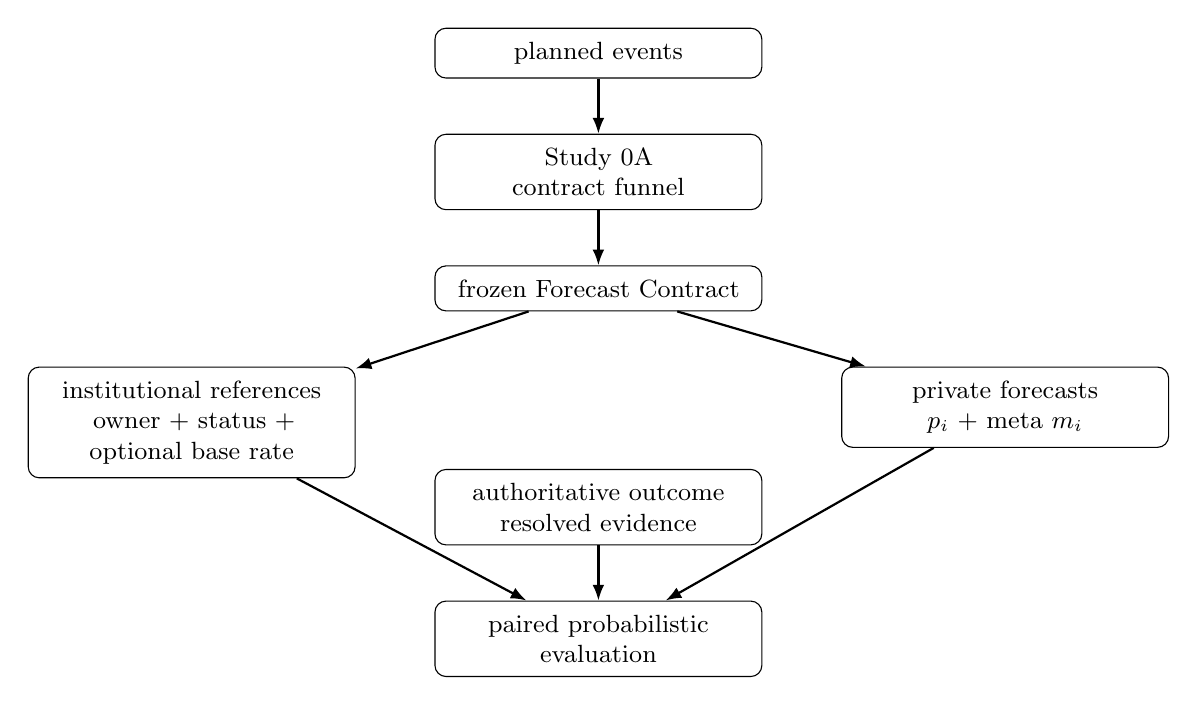
\begin{tikzpicture}[
  node distance=7mm and 10mm,
  box/.style={draw, rounded corners, align=center, inner sep=5pt, text width=3.8cm, font=\small},
  arrow/.style={-{Latex[length=2mm]}, thick}
]
\node[box] (cand) {planned events};
\node[box, below=of cand] (funnel) {Study 0A\\contract funnel};
\node[box, below=of funnel] (contract) {frozen Forecast Contract};
\node[box, below left=of contract] (inst) {institutional references\\owner + status + optional base rate};
\node[box, below right=of contract] (crowd) {private forecasts\\$p_i$ + meta $m_i$};
\node[box, below=20mm of contract] (outcome) {authoritative outcome\\resolved evidence};
\node[box, below=of outcome] (analysis) {paired probabilistic\\evaluation};
\draw[arrow] (cand) -- (funnel);
\draw[arrow] (funnel) -- (contract);
\draw[arrow] (contract) -- (inst);
\draw[arrow] (contract) -- (crowd);
\draw[arrow] (inst) -- (analysis);
\draw[arrow] (crowd) -- (analysis);
\draw[arrow] (outcome) -- (analysis);
\end{tikzpicture}
\caption{Minimum-sufficient Study~0 sequence. No aggregate is exposed before resolution.}
\end{figure}

\subsection{Frozen elements}
Table~\ref{tab:freeze} summarizes the minimum prospective freeze.

\begin{table}[ht]
\centering
\small
\begin{tabular}{p{0.28\linewidth}p{0.62\linewidth}}
\toprule
Element & Frozen content \\
\midrule
Event & question, binary outcome, cluster, open/close/resolve times \\
Resolution & authoritative evidence, rule, resolver and ambiguity handling \\
Institutional reference & base-rate availability/rule, owner role and official-status source \\
Participants & eligibility, actor/observer quotas, abstention and AI-assistance metadata \\
Aggregation & raw mean/median plus fixed meta-belief rule and constants \\
Analysis & Brier convention, estimands, cluster bootstrap, stopping and continuation rule \\
Safeguards & data custodian, pre-resolution visibility prohibitions and no-HR-use controls \\
\bottomrule
\end{tabular}
\caption{Elements fixed before outcome inspection.}
\label{tab:freeze}
\end{table}

\subsection{Actor and observer as a design factor}
Forecasts about one's own task can differ systematically from observer forecasts; planning-fallacy work documents actor/observer asymmetries in completion-time judgments \citep{buehler1994}. Study~0 therefore preregisters participation composition and reports actor-only and observer-only aggregates, rather than treating influence over the outcome as optional metadata.

\subsection{Primary private collective aggregator}
For clipped probabilities in $[0.01,0.99]$, define
\[
L_i=\logitop(p_i),\qquad M_i=\logitop(m_i).
\]
With
\[
\bar L=\frac1n\sum_iL_i,\qquad
\bar M=\frac1n\sum_iM_i,
\]
the default protocol uses the fixed transform
\[
p^{\mathrm{crowd}}=\sigmoid\!\left(\bar M+a(\bar L-\bar M)\right),\qquad a=2.
\]
The constant is frozen before outcomes and is not tuned on Study~0. Mean and median remain required comparators. The transform is a project implementation motivated by meta-belief/shared-information literature \citep{palley2019,peker2025}, not an assertion that it is their exact published algorithm.

\section{Scoring and estimands}
For binary outcome $y_j\in\{0,1\}$ this repository uses
\[
\BS(p,y)=(p-y)^2.
\]
This is the normalized one-component binary quadratic/Brier loss. Brier's original two-category vector sum is twice this quantity for a binary event; the repository uses the convention above consistently \citep{brier1950,gneiting2007}.

The primary paired contrast is
\[
\Delta_j^{\mathrm{owner}}
=
\BS\!\left(p_j^{\mathrm{crowd}},y_j\right)
-
\BS\!\left(p_j^{\mathrm{owner}},y_j\right).
\]
For contracts with a defensible prospectively frozen base rate, the required reference contrast is
\[
\Delta_j^{\mathrm{base}}
=
\BS\!\left(p_j^{\mathrm{crowd}},y_j\right)
-
\BS\!\left(p_j^{\mathrm{base}},y_j\right).
\]
Each otherwise-admissible resolved contract receives equal weight in the primary crowd-versus-owner estimand; $\Delta^{\mathrm{base}}$ is reported on the explicitly enumerated base-rate-available subset. Cluster identifiers are assigned prospectively when contracts share an operational episode; bootstrap resampling occurs at that cluster level.

\subsection{Why the mean remains useful}
For the arithmetic mean $\bar p$,
\[
\BS(\bar p,y)
=
\frac1n\sum_i \BS(p_i,y)
-
\frac1n\sum_i(p_i-\bar p)^2.
\]
The identity shows how disagreement can improve the squared-error performance of an average relative to average individual error. It does not imply that probability averaging fully pools independent evidence.

\subsection{Calibration and sample size}
Calibration and sharpness are reported descriptively at Study~0 scale. The default continuation gate uses $J_{min}=30$, $K_{min}=8$ and $\delta_{NI}=0.02$ on the normalized Brier-loss scale unless a deployment freezes different values before Study~0A begins. At this scale the gate is deliberately a screening/non-inferiority rule: it can reject a crowd that is clearly worse than the owner but cannot establish that the crowd is better. If reliable discrimination near equality is required, a larger $J$ must be planned prospectively rather than widening the margin after outcomes.

\section{Design operating characteristics}

The structural target of approximately 30 resolved contracts is not presented as a conventional power calculation for superiority. To make the continuation rule more interpretable before data collection, an independent design review evaluated toy operating characteristics for the rule
\[
\mathrm{UCB}_{0.975}\!\left(\overline{\Delta}^{\mathrm{owner}}\right)\le \delta_{NI},
\qquad \delta_{NI}=0.02,
\]
where the upper bound is obtained by cluster bootstrap. The simulation uses $J=32$ contracts so that equal clusters can be formed for both $K=8$ and $K=16$. Outcomes follow a Bernoulli process with prevalence 0.65; six forecasters receive a mixture of public and conditionally independent private signals; reported logits and meta-predictions are noisy; and the crowd uses the preregistered $a=2$ meta-recalibration. Three owner configurations represent an optimistic actor, an unbiased one-signal owner and a better-informed four-signal owner. Contracts are independent across clusters, an optimistic assumption.

Table~\ref{tab:continuation-oc} reports the probability that the continuation rule is met under the protocol-candidate margin $\delta_{NI}=0.02$. The values are Monte Carlo design evidence, not observations from an engineering organization.

\begin{table}[ht]
\centering
\small
\begin{tabular}{llrrr}
\toprule
Information regime & Owner model & $E[\Delta_{\mathrm{owner}}]$ & $K=8$ & $K=16$ \\
\midrule
Mostly private & optimistic actor & $-0.065$ & 78\% & 75\% \\
Mostly private & unbiased & $-0.060$ & 72\% & 72\% \\
Mostly private & well informed & $+0.016$ & 5\% & 4\% \\
Mostly shared & optimistic actor & $-0.014$ & 53\% & 47\% \\
Mostly shared & unbiased & $-0.010$ & 52\% & 47\% \\
Mostly shared & well informed & $+0.004$ & 17\% & 14\% \\
\bottomrule
\end{tabular}
\caption{Toy operating characteristics at $J=32$ and $\delta_{NI}=0.02$. Entries in the last two columns are the simulated probability of satisfying the Study~0B continuation rule. Negative $\Delta_{\mathrm{owner}}$ favors the private crowd.}
\label{tab:continuation-oc}
\end{table}

The simulation supports a deliberately narrow interpretation of the minimum scale. When the crowd is clearly better in the toy mostly-private regime, the rule continues in roughly 72--78\% of simulated studies. When the owner is better, continuation falls to 4--17\% in the configurations shown. Near equality or modest crowd advantage is difficult to distinguish: continuation is only about 47--53\% in the mostly-shared one-signal-owner cases. Larger margins of 0.05 or 0.08 made the rule substantially more permissive in the same simulation and are therefore not substituted after observing Study~0 data.

Consequently, $J_{\min}=30$, $K_{\min}=8$ and $\delta_{NI}=0.02$ define a \emph{screening/non-inferiority continuation gate}. They do not provide 80\% power for a superiority claim and do not establish that 30 contracts are universally sufficient. A deployment that requires reliable discrimination near equality must prospectively increase the target sample rather than reinterpret a null or widen the margin after outcomes.

The exact reviewer-supplied simulation code, frozen seeds and reference outputs are retained under \texttt{analysis/design\_simulation/}. The simulation's purpose is transparency about the gate's behavior under explicit assumptions; it is not part of the empirical Study~0 evidence base.

\section{Organizational safeguards}
Private forecasting concerns employee judgments and operational knowledge. Study~0 therefore requires voluntary participation, an independent data custodian, pseudonymous analysis, no real-money mechanism, data minimization, non-retaliation for pessimistic forecasts, no individual HR use and no pre-resolution aggregate access by participants or decision owners.

The no-HR-use rule includes longitudinal forecaster track records. Raw rationales are excluded by default because they can reveal confidential architecture, personnel or project information.

\paragraph{Use of AI assistants and EU AI Act boundary.}
A participant may consult an AI assistant only as a declared ancillary information source and through an organization-approved usage path. The study records whether an assistant was consulted and, where policy permits, a coarse assistance category; prompts, confidential transcripts and proprietary engineering evidence are not copied into the public research dataset. AI output is non-authoritative: the participant remains responsible for the submitted probability, and authoritative engineering evidence remains the Forecast Contract resolution source. Regulation (EU) 2026/1744, in force since 27~July~2026, replaced Article~4 of the EU AI Act: providers and deployers must take measures to \emph{support the development} of AI literacy among staff and other persons using AI systems on their behalf, without having to guarantee any specific level for an individual \citep{euai2026}. Article~50 applies from 2~August~2026; for systems already placed on the market before that date, the limited transition for the Article~50(2) marking/detection obligation runs until 2~December~2026 \citep{ec2026transparency}. The protocol does not classify ordinary assistant use as high-risk by default; however, if AI outputs or forecasting records were repurposed to monitor or evaluate workers, allocate tasks, or influence employment decisions, a separate legal classification would be required and the employment use cases in Annex~III could become relevant. This is one reason the study prohibits individual HR use.

Private elicitation can still trigger reflection. The study therefore records \emph{detected} interference. Otherwise resolvable contracts remain in the intention-to-observe primary analysis; excluding detected material interference is a preregistered sensitivity analysis rather than a post-treatment void rule.

\section{Claims and gates}
Study~0 maintains a bounded claim ladder:

\begin{description}[leftmargin=2.15cm,style=nextline]
\item[C0A Contract funnel] Can real events be prospectively specified and later resolved cleanly?
\item[C0B Private feasibility] Can same-time private forecasts and institutional references be collected with acceptable burden and no detected material interference?
\item[C1 Incremental signal] What is the paired crowd-versus-owner Brier difference, with base-rate skill reported where a defensible reference class exists?
\item[C2 Aggregation] Exploratorily, how does fixed meta-belief recalibration compare with raw mean/median?
\item[C3 Information structure] Exploratorily, how do actor/observer status and information locality relate to error?
\item[C4 Market residual value] Future study only.
\end{description}

\section{Threats to validity}
\paragraph{Construct validity.}
A precise Forecast Contract can still target an unimportant or gameable event. Official status is not itself a probability unless a mapping was frozen.

\paragraph{Internal validity.}
Private elicitation can change attention; actors can differ from observers; common data or common AI assistance can correlate forecasts; question wording can leak expectations.

\paragraph{Statistical validity.}
The number of independent contracts/clusters may be small, event families may be imbalanced, and exploratory comparisons can multiply. Cluster-level resampling and prospective funnel registration address only part of these limitations.

\paragraph{External validity.}
Results from one organization, calendar period or event family require replication. Corporate market evidence does not transfer automatically to engineering private polls.

\paragraph{Causal validity.}
Forecast performance is not a causal treatment effect. Conditional predictions do not become interventional quantities without a causal design.

\section{Why prediction markets move to a later study}
The minimum-sufficient-mechanism test asks what can be removed without losing the ability to answer the current research question. A private poll can test whether distributed knowledge adds signal beyond institutional baselines without exposing a social aggregate. A market adds price visibility, liquidity, mechanism parameters and behavioral feedback. Study~0 therefore removes it.

A later Study~2 may compare a prediction market against a qualified private aggregator at the same information time, using either an observers-only arm or an explicitly intervention-aware design. That study would test \emph{residual market value}, not conflate market mechanics with later information or recalibration.

\section{Research roadmap}
\textbf{Study~0A} qualifies the event/contract funnel. \textbf{Study~0B} estimates private collective skill beyond institutional references. \textbf{Study~1} replicates and qualifies private aggregation methods. After Study~1, two branches become possible: \textbf{Study~2} may test residual prediction-market value, while \textbf{Study~3} may independently study whether exposing qualified private forecast evidence changes evidence acquisition or real decisions. Study~3 does not depend on Study~2; a prediction market is not on the critical path to operational-value research. Human--machine combinations are deferred until an independently qualified model exists.

A later sequential-decision programme may treat a collective forecast as one observation or elicitation as an information-acquisition action. That possible bridge is not needed to justify Study~0.

\section{Pedagogical and knowledge-base boundary}
Reusable concepts are capitalized separately in the Diderot MMALS/ML knowledge repository:
\url{https://github.com/gharbonnier78/mmals-ml-wiki}.
The teaching layer explains concepts and provenance; it is not scientific authority for this project's empirical claims.

\section{Data and code availability}
Protocol source, schemas, reference analysis code and synthetic templates are maintained at:
\url{https://github.com/gharbonnier78/engineering-collective-forecasting}.
A scientific report must cite the immutable commit actually used. Internal participant data and proprietary engineering evidence are not part of the public repository.

\section{Conclusion}
The revised protocol deliberately tests the smallest mechanism that can answer the immediate question. First, establish that engineering events can be specified and resolved prospectively. Second, compare a private collective forecast with the organization's own same-time reference signals. Only then ask whether a prediction market, machine model or decision intervention adds residual value. The intended output of Study~0 is not a release gate; it is evidence about whether distributed engineering knowledge can be measured as a disciplined probabilistic signal.


\bibliographystyle{plainnat}
\bibliography{references}
\end{document}
